\section{Modeling error}

The modeling error, also known as the residual, is calculated as the disparity between the system output and the model output generated with the same input.
\begin{figure}[H]
    \centering
    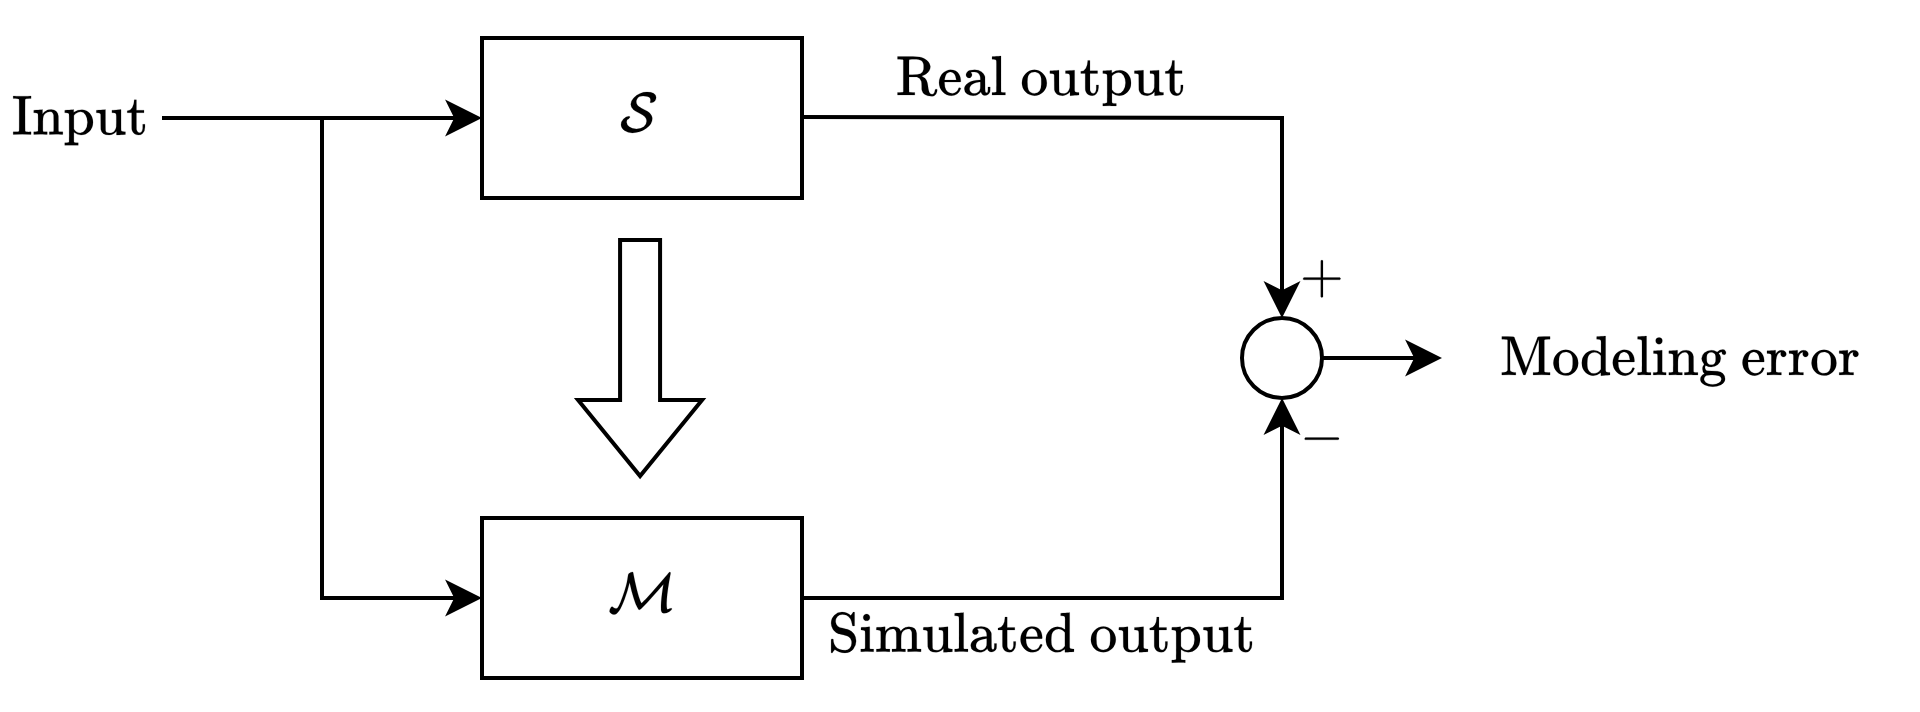
\includegraphics[width=0.7\linewidth]{images/error.png}
\end{figure}
When the outputs exhibit similarity based on certain metrics, it signifies that the model accurately mirrors the dynamics of the system. 
However, if patterns persist within the error graph, it indicates that not all information has been effectively extracted from the data. 
Conversely, if the error graph lacks of patterns, it is termed as  White Noise, suggesting an inability to extract further meaningful information from the data.
\begin{definition}[\textit{Complete model}]
    A model is deemed complete only when the error demonstrates a completely unpredictable pattern.
\end{definition}